\documentclass[10pt]{beamer}
\usetheme{SimplePlus}
\usepackage[T1]{fontenc}
\usefonttheme[onlymath]{serif}

\usepackage{amssymb,amsmath,mathtools,stmaryrd}
\usepackage{graphicx}
\usepackage[export]{adjustbox}
\usepackage[font=scriptsize,labelfont=scriptsize]{caption}
\usepackage{tikz}
\graphicspath{{../../Koornwinder_polynomials/}{../Example of previous presentation/}}

% Colors (as in the previous talk)
\definecolor{uibred}  {HTML}{db3f3d}
\definecolor{uibblue} {HTML}{4ea0b7}
\definecolor{uibgreen}{HTML}{5e8340}
\definecolor{uiblink2}{HTML}{004f6a}
\definecolor{blue}{RGB}{40,68,104}
\setbeamercolor{alerted text}{fg=uibred}
\newcommand{\rstar}{\textcolor{uibred}{\boldsymbol{\ast}}}
\newcommand{\semitransp}[2][35]{\textcolor{fg!#1}{#2}}

% Notation of the paper
\newcommand{\ZZ}{\mathbb Z}
\newcommand{\QQ}{\mathbb Q}
\newcommand{\KK}{\mathbb K}
\newcommand{\Sign}{\mathrm{Sign}}
\newcommand{\hb}[1]{\overline{#1}}
\DeclareMathOperator{\wt}{wt}
\DeclareMathOperator{\skipped}{skip}
\DeclareMathOperator{\free}{free}
\DeclareMathOperator{\lb}{lb}
\DeclareMathOperator{\Top}{Top}
\newcommand{\conf}[2][2]{%
  \begingroup
  \renewcommand{\arraystretch}{1.25}%
  \left[
  \begin{array}{@{\;}c*{\numexpr#1-1\relax}{@{\quad}c}@{\;}}
  #2
  \end{array}
  \right]%
  \endgroup
}

% Title page: SimplePlus template with a smaller top space (6em -> 2.5em)
\makeatletter
\setbeamertemplate{title page}{%
    \vspace{2.5em}
    \begingroup
    \centering
    \begin{beamercolorbox}[sep=10pt,center]{title}
        \usebeamerfont{title}\inserttitle\par%
        \ifx\insertsubtitle\@empty%
        \else%
        \vskip0.25em%
        {\usebeamerfont{subtitle}\usebeamercolor[fg]{subtitle}\insertsubtitle\par}%
        \fi%
    \end{beamercolorbox}%
    \vskip0.5em\par
    \begin{beamercolorbox}[sep=8pt,center]{author}
        \usebeamerfont{author}\insertauthor
    \end{beamercolorbox}
    \vskip-1em
    \begin{beamercolorbox}[sep=8pt,center]{institute}
        \usebeamerfont{institute}\insertinstitute
    \end{beamercolorbox}
    \begin{beamercolorbox}[sep=8pt,center]{date}
        \usebeamerfont{date}\insertdate
    \end{beamercolorbox}\vskip0.5em
    {\usebeamercolor[fg]{titlegraphic}\inserttitlegraphic\par}
    \endgroup
    \vfill
}
\makeatother

\title[Two-row recurrence for Koornwinder polynomials]{Two-row recurrence for Koornwinder polynomials}
\author[Houcine Ben Dali]{Houcine Ben Dali}
\institute{Harvard University\\[1.8em]
  {\large joint work with Lauren Williams}}
\setbeamerfont{author}{size=\large}
\setbeamerfont{institute}{size=\small}
\setbeamerfont{date}{size=\small}
\date{{\large\textcolor{uiblink2}{Conférence en l'honneur de Philippe Biane}}\\[0.4em]
  Paris, Sorbonne Université\\[0.2em]
  October 19, 2026}

\begin{document}
\begin{frame}{Option 1: three children, type $A$ in the middle}
\centering
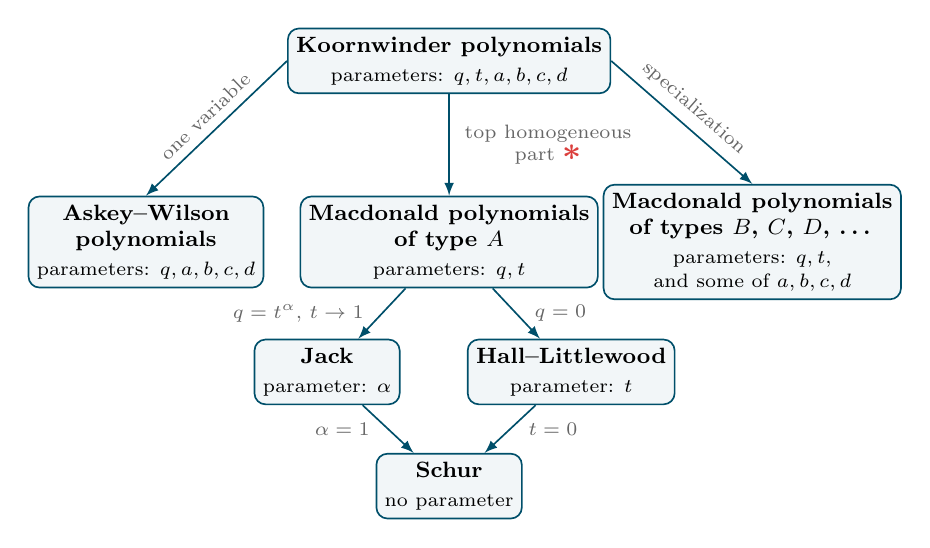
\begin{tikzpicture}[
  fam/.style={draw=uiblink2,rounded corners,line width=0.6pt,fill=uiblink2!5,align=center,inner sep=3pt,font=\footnotesize},
  arr/.style={-latex,line width=0.6pt,uiblink2},
  lab/.style={font=\scriptsize,text=black!60,align=center},
  dim/.style={},
  hot/.style={}]
  \node[fam] (K) at (0,0) {\textbf{Koornwinder polynomials}\\[1pt] {\scriptsize parameters: $q,t,a,b,c,d$}};
  \node[fam,dim] (AW) at (-3.85,-2.3) {\textbf{Askey--Wilson}\\ \textbf{polynomials}\\[1pt] {\scriptsize parameters: $q,a,b,c,d$}};
  \node[fam] (A) at (0,-2.3) {\textbf{Macdonald polynomials}\\ \textbf{of type $A$}\\[1pt] {\scriptsize parameters: $q,t$}};
  \node[fam,dim] (BC) at (3.85,-2.3) {\textbf{Macdonald polynomials}\\ \textbf{of types $B$, $C$, $D$, \dots}\\[1pt] {\scriptsize parameters: $q,t$,}\\[-1pt] {\scriptsize and some of $a,b,c,d$}};
  \node[fam] (J) at (-1.55,-3.95) {\textbf{Jack}\\[1pt] {\scriptsize parameter: $\alpha$}};
  \node[fam] (HL) at (1.55,-3.95) {\textbf{Hall--Littlewood}\\[1pt] {\scriptsize parameter: $t$}};
  \node[fam] (S) at (0,-5.4) {\textbf{Schur}\\[1pt] {\scriptsize no parameter}};
  \draw[arr,dim] (K.west) -- node[lab,sloped,above] {one variable} (AW.north);
  \draw[arr,hot] (K) -- node[lab,right=2pt] {top homogeneous\\ part {\large$\rstar$}} (A);
  \draw[arr,dim] (K.east) -- node[lab,sloped,above] {specialization} (BC.north);
  \draw[arr] (A) -- node[lab,left=3pt] {$q=t^\alpha$, $t\to1$} (J);
  \draw[arr] (A) -- node[lab,right=3pt] {$q=0$} (HL);
  \draw[arr] (J) -- node[lab,left=3pt] {$\alpha=1$} (S);
  \draw[arr] (HL) -- node[lab,right=3pt] {$t=0$} (S);
\end{tikzpicture}
\vfill
{\raggedright\scriptsize {\large$\rstar$} Symmetric case: van Diejen (1995). Nonsymmetric case: BD--Williams.\par}
\end{frame}
\begin{frame}{Option 2: type $A$ branch in focus}
\centering
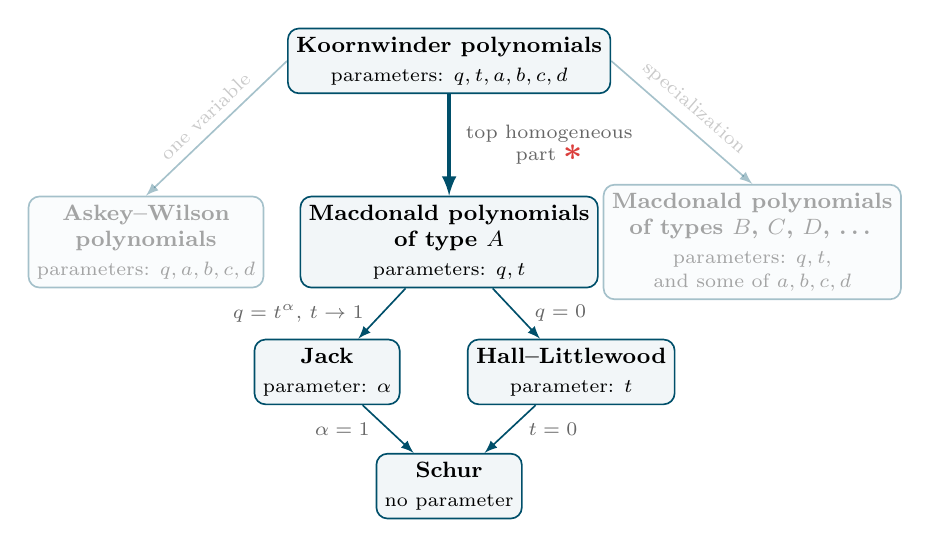
\begin{tikzpicture}[
  fam/.style={draw=uiblink2,rounded corners,line width=0.6pt,fill=uiblink2!5,align=center,inner sep=3pt,font=\footnotesize},
  arr/.style={-latex,line width=0.6pt,uiblink2},
  lab/.style={font=\scriptsize,text=black!60,align=center},
  dim/.style={opacity=0.35,},
  hot/.style={line width=1.4pt}]
  \node[fam] (K) at (0,0) {\textbf{Koornwinder polynomials}\\[1pt] {\scriptsize parameters: $q,t,a,b,c,d$}};
  \node[fam,dim] (AW) at (-3.85,-2.3) {\textbf{Askey--Wilson}\\ \textbf{polynomials}\\[1pt] {\scriptsize parameters: $q,a,b,c,d$}};
  \node[fam] (A) at (0,-2.3) {\textbf{Macdonald polynomials}\\ \textbf{of type $A$}\\[1pt] {\scriptsize parameters: $q,t$}};
  \node[fam,dim] (BC) at (3.85,-2.3) {\textbf{Macdonald polynomials}\\ \textbf{of types $B$, $C$, $D$, \dots}\\[1pt] {\scriptsize parameters: $q,t$,}\\[-1pt] {\scriptsize and some of $a,b,c,d$}};
  \node[fam] (J) at (-1.55,-3.95) {\textbf{Jack}\\[1pt] {\scriptsize parameter: $\alpha$}};
  \node[fam] (HL) at (1.55,-3.95) {\textbf{Hall--Littlewood}\\[1pt] {\scriptsize parameter: $t$}};
  \node[fam] (S) at (0,-5.4) {\textbf{Schur}\\[1pt] {\scriptsize no parameter}};
  \draw[arr,dim] (K.west) -- node[lab,sloped,above] {one variable} (AW.north);
  \draw[arr,hot] (K) -- node[lab,right=2pt] {top homogeneous\\ part {\large$\rstar$}} (A);
  \draw[arr,dim] (K.east) -- node[lab,sloped,above] {specialization} (BC.north);
  \draw[arr] (A) -- node[lab,left=3pt] {$q=t^\alpha$, $t\to1$} (J);
  \draw[arr] (A) -- node[lab,right=3pt] {$q=0$} (HL);
  \draw[arr] (J) -- node[lab,left=3pt] {$\alpha=1$} (S);
  \draw[arr] (HL) -- node[lab,right=3pt] {$t=0$} (S);
\end{tikzpicture}
\vfill
{\raggedright\scriptsize {\large$\rstar$} Symmetric case: van Diejen (1995). Nonsymmetric case: BD--Williams.\par}
\end{frame}
\end{document}
